\documentclass[12pt]{article}
\usepackage[letterpaper,margin=1in]{geometry}
\usepackage[T1]{fontenc}
\usepackage{mathptmx}
\usepackage{amsmath,amssymb,amsthm}
\usepackage{graphicx}
\usepackage{booktabs,array,tabularx}
\usepackage[table]{xcolor}
\usepackage{float}
\usepackage{needspace}
\usepackage[hang,flushmargin]{footmisc}
\usepackage{caption}
\usepackage{titlesec}
\usepackage{xurl}
\usepackage[colorlinks=true,linkcolor=black,citecolor=black,urlcolor=black]{hyperref}

% ---- JAI/PMR mechanical standards: single spacing, 12pt before paragraphs, tab indent ----
\setlength{\parskip}{12pt}
\setlength{\parindent}{0.5in}
\setlength{\emergencystretch}{3em}

% ---- headings: top level bold uppercase, second level indented bold, third level bold run-in ----
\titleformat{\section}{\normalfont\bfseries}{\thesection.}{0.5em}{\MakeUppercase}
\titleformat{\subsection}{\normalfont\bfseries}{\thesubsection.}{0.5em}{}
\titlespacing*{\subsection}{0.5in}{12pt}{0pt}
\titleformat{\subsubsection}[runin]{\normalfont\bfseries}{\thesubsubsection.}{0.5em}{}[.]
\titlespacing*{\section}{0pt}{18pt}{6pt}

% ---- all tables and figures are "Exhibits", numbered consecutively, title above ----
\makeatletter
\let\c@table\c@figure
\makeatother
\renewcommand{\thetable}{\arabic{figure}}
\captionsetup{labelsep=colon,skip=6pt}
\captionsetup[figure]{name=Exhibit,position=top}
\captionsetup[table]{name=Exhibit,position=top}

% ---- revision marking: all added or changed text is set in blue ----
\DeclareRobustCommand{\chg}[1]{{\color{blue}#1}}
\definecolor{blue}{rgb}{0,0,0}

\theoremstyle{plain}
\newtheorem{identity}{\color{blue}Identity}
\newtheorem{observation}{\color{blue}Observation}
\newtheorem{proposition}{\color{blue}Proposition}
\newtheorem{propA}{\color{blue}Proposition}
\renewcommand{\thepropA}{A.\arabic{propA}}
\newtheorem{propB}{\color{blue}Proposition}
\renewcommand{\thepropB}{B.\arabic{propB}}
\theoremstyle{remark}
\newtheorem{remark}{Remark}

\newcommand{\Vref}{V^{\mathrm{ref}}}
\newcommand{\Vsubj}{V^{\mathrm{subj}}}
\newcommand{\ceff}{c_{\mathrm{eff}}}
\newcommand{\E}{\mathbb{E}}

\title{Bitcoin's Expected Return: An Age Rule That Beats Current Practice}
\author{Agisilaos Papadogiannis\thanks{Independent Researcher (PhD, MBA). \textit{Correspondence:} apapadogiannis@gmail.com. \textit{ORCID:} 0009-0002-7753-7052. Data, code and replication files: \url{https://github.com/apapadogiannis/bitcoin-age-rule}, archived at \url{https://doi.org/10.5281/zenodo.24004326}.}}
\date{November 2026}

\begin{document}
\maketitle

\begin{abstract}
\noindent Investors need a long-run expected return for Bitcoin, but there is no established way to set one. In practice it comes from scenario models, as in the capital market assumptions J.P. Morgan has just extended to Bitcoin, or from Bitcoin's own past growth. We test both as forecasts against the returns that followed over rolling three- to five-year periods since 2012, with gold as a control and Ether as a younger comparison. Both fail: every constant rate from 7\% to 21\% a year, a range covering J.P. Morgan's assumption, was beaten in about nine periods in ten, by 70--120 points a year on average, while Bitcoin's long-run average growth was almost never beaten. A simple age rule comes closest: in log terms, Bitcoin's expected return is about 5.6 divided by its age in years, a forecast of about 32\% a year for September 2026 to 2031, far above a CAPM required return and what crypto holders say they expect. Gold's record fits every candidate from inflation plus 1\% to 7\%; Ether's is too short to test.
\end{abstract}

\noindent{\large\bfseries Highlights}
\vspace{-6pt}
\begin{itemize}
\item Of all the candidates, an age rule comes closest to Bitcoin's expected return: in log terms, about 5.6 divided by its age in years, or a forecast of about 32\% a year for September 2026 to 2031.
\item The rates used in practice fail as forecasts: rates of 7--21\%, the level at which J.P. Morgan's new assumption sits, were beaten in about nine three- to five-year periods in ten since 2012, and Bitcoin's own long-run average growth in almost none.
\item The age rule's 32\% forecast exceeds both a CAPM required return of 6--18\% and the 14--22\% that crypto holders report expecting; gold's history fits every candidate from inflation plus 1\% to 7\%, and Ether's is too short to test.
\end{itemize}

% ============================ MAIN TEXT ============================
\section{Introduction}\label{sec:intro}

Anyone building a portfolio needs a long-run expected return for each asset, and for Bitcoin there is no good way to get one. For equities there is a century of data, an accepted theory of the risk premium and valuation ratios to check it against, and even so the estimate is imprecise (Fama and French 1997, 2002). Bitcoin has fifteen years of data, no close comparable, returns that barely move with the factors that price stocks (Liu and Tsyvinski 2021), and equilibrium models of its price (Biais et al.\ 2023; Pagnotta 2022; Cong, Li, and Wang 2021) that have not been calibrated to a long-run expected return. In practice the number comes from scenario models, as in the capital market assumptions that J.P. Morgan Asset Management (2026) has just extended to Bitcoin, or from Bitcoin's own price history, as in the trend models that commentators follow (PlanB 2019; Burger 2019). The power law behind one of those models has been studied as a description and forecast of the price (Burger and Vijn 2024; Baquero and Menezes 2026; \c{S}enel and Y{\i}lmaz 2026). What has not been done is to test the expected-return assumptions themselves against the returns that followed. This paper does that.

The test is a backtest: set each candidate rate with the information available at the time, wait three to five years, and compare it with what Bitcoin earned, on average over all such periods since 2012. The rates used in practice fail in both directions. Rates of 7--21\%, the level at which institutional assumptions sit, were far too low; Bitcoin's own long-run average growth was far too high. A simple rule, which we call the age rule, comes closest: in log terms, Bitcoin's expected return is its power-law exponent, about 5.6, divided by its age in years, which today forecasts about 32\% a year for September 2026 to 2031. The age rule is implicit in the power-law model of Bitcoin's price published by Burger (2019), so the claim is not that this paper forecasts Bitcoin better than the model's authors, but that a rate implicit in a public model beats the rates institutions use. It is not a curve-fitting accident: Bitcoin's price has reverted to the trend, the exponent has been stable, and the age rule did not break in the periods that began after the model was published.

The age rule's 32\% is far above a CAPM required return of 6--18\%, and above the 14--22\% that holders of crypto report expecting. Neither gap has an explanation yet. The CAPM's premise does not fit Bitcoin, whose returns barely load on the factors that price stocks, and the equilibrium models of its price have not been asked what return its holders should require. This paper supplies the three numbers any such account has to fit: a tested expected return, a CAPM required return, and what holders say they expect.

Gold and Ether show what the test can and cannot do. Gold is the control: two centuries of prices and a literature built on them put its expected return at about 1\% a year above inflation, about 4.4\% today (Barro and Misra 2016; Erb and Harvey 2013), so the answer is known before the backtest runs. The backtest agrees with it: since 1981 gold's returns have averaged within three points a year of every candidate with a case of its own, from inflation plus 1\% through its CAPM rate of about 5.5\% to the 7\% often assumed, so all of them pass, and 45 years of data cannot rank rates that close. That calibrates the Bitcoin results: a test that cannot tell 4\% from 7\% for gold rejects the institutional rates for Bitcoin by 70--120 points a year. Ether is the same test applied to a younger asset, and its history is too short to validate any rule, the age rule included. How much a price history reveals depends on how long it is relative to how fast the asset is maturing.\footnote{This paper applies the separation of an asset's expected return from the investor's required return developed in the author's dual-risk framework (Papadogiannis 2026a, 2026b, 2027), but uses none of that framework's apparatus; the framework needs a discount rate and does not say how to estimate one for an asset without a close comparable.}

Section~\ref{sec:setc} separates the expected return from the required return. Section~\ref{sec:design} describes the test, Section~\ref{sec:calibsec} reports what works for Bitcoin, and Section~\ref{sec:formula} asks whether the age rule is more than a fitted curve. Section~\ref{sec:required} compares it with the required return, Section~\ref{sec:gold} turns to gold and Ether, Section~\ref{sec:practice} draws the implications, and Section~\ref{sec:conclusion} concludes. Appendix~A gives data sources, statistical details and robustness results.

\section{Two Returns, Two Practices}\label{sec:setc}

Two returns matter for any investment, and for assets such as gold and Bitcoin they are easily confused. The \emph{expected return} is a forecast: what the asset will earn on average. For an asset that pays no income it is the rate $c$ at which its price is expected to grow, $\E_t[P_{t+h}]=P_t(1+c)^h$ over a horizon of $h$ years, and realized returns are the only check on it (Elton 1999). The \emph{required return} is a hurdle: what an investor needs the asset to earn to compensate for its risk, the return available elsewhere for bearing the same risk (Sharpe 1964; Lintner 1965). In a valuation it is the discount rate. The first is a property of the asset's price process; the second is a demand the investor brings to it, and the two need not coincide (Papadogiannis 2026b).

Allocation turns on the gap between the two, which is the logic of Black and Litterman (1992): the market's weights embed the required returns, an investor's forecasts are the expected returns, and the tilt away from the market is proportional to the difference. An investor who expects Bitcoin to earn 30\% a year but requires only 10\% for its risk should hold more of it than the market as a whole does; one who expects exactly the required return has no reason to depart from the market's weighting; one who expects less should hold less, or none. Equilibrium models assume the two returns coincide, which is why studies of mature assets often treat them as one; whether they do is an empirical question, and for an asset still being repriced as it is adopted they can differ for years.

Without a close comparable, both returns are hard to pin down, and practice often uses one number for both. Three routes are common. The first sets a rate at the level of comparable assets, a broad equity index, growth stocks or gold, on the argument that Bitcoin should earn roughly what such assets earn. That is a statement about the required return, true only if the assets carry comparable risk, yet the rate is used as the expected return. The second forecasts the expected return from the asset's own history, as commentator models do (PlanB 2019; Burger 2019), either by extrapolating past growth or by assuming that growth keeps slowing. The third builds scenarios and converts them into a price path. J.P. Morgan Asset Management (2026), which describes Bitcoin as trading ``like a high beta risk asset'' that is ``sometimes treated as digital gold,'' blends a money-supply model, a scenario in which Bitcoin complements gold and an adoption model to arrive at 10\% a year compound, 21\% arithmetic, above its 5.5\% for gold and 7.5\% for US large-cap equities, while noting the difficulty of ``forecasting an asset whose fundamentals are not cash flows.'' Adoption scenarios, such as Bitcoin capturing a share of gold's market or of central-bank reserves, are too recent to test and disagree widely, from 15--34\% a year (Selby 2025; Sigel 2026; Bitwise Asset Management 2026) to $-3$\% in J.P. Morgan's own network-adoption framework. Whatever the route, the institutional figures land at the level of comparable assets, 7--21\% a year, and that is the range the next sections test.

Only expected returns can be checked against what happened, so the next sections test every candidate as a forecast. A rate that fails was a poor forecast, but not necessarily the wrong hurdle: an asset that stayed cheap for years would beat a correct hurdle. Section~\ref{sec:required} returns to the required return.

\section{The Test}\label{sec:design}

In every month, set a candidate expected return using only what was known at the time, wait $h$ years, and compare it with what the asset actually earned. We use monthly prices for Bitcoin from August 2010, Ether from August 2015, gold from 1971 and the S\&P 500 total-return index from 1871, all to September 2026 (April 2026 for Ether), with US consumer prices and Treasury yields; Appendix~A.1 lists the sources. Gold serves as a control, an asset whose expected return is known from a long record, and Ether as a younger asset on which the same methods can be tried. Throughout this section $c$ is a candidate forecast of the expected return, not a hurdle. For a candidate $c$ and a horizon of $h\in\{3,4,5\}$ years, the ratio of the price reached to the price the rate implied,
\begin{equation}
\widehat{G}_{t,h}(c)=\frac{P_{t+h}}{P_t(1+c)^h}, \label{eq:Khat5}
\end{equation}
is above one when the asset beat the rate and below one when it fell short.

A good forecast is right on average, not in every period: if $c$ is correct, $\E_t[\widehat{G}_{t,h}(c)]=1$, the standard check of expected-return estimates (Fama and French 2002). We therefore report each rate's \emph{average miss}, $\bar{G}^{1/h}-1$, the annual return by which the asset beat the rate on average. For a volatile asset, being right on average looks odd period by period: a few spectacular periods pull the average up, so a correct expected return is beaten in a minority of periods, about 45\% of them for gold but only 17--34\% for Bitcoin (Appendix~A.3). A rate that Bitcoin beat half the time is closer to its median return, which lies well below its average.

The mean and the median differ because volatility drags on compounding: an investment that goes from 100 to 200 and back to 100 has returned $+100$\% and then $-50$\%, an average of 25\% a year, yet the money has compounded at 0\%. The arithmetic average of yearly returns exceeds the compound rate by about half the variance, under a point a year for gold but 10--15 points for Bitcoin. Since the expected price is pulled up by the lucky paths, $c$, the rate that grows to the expected price, is the arithmetic-type figure; a practitioner's compound assumption corresponds to a higher $c$, which is why J.P. Morgan's 10\% compound is 21\% arithmetic, and 21\% is the number to test. We report the median miss and the share of periods in which the asset beat the rate alongside the average.

With so short a history, chance matters. Rolling periods overlap, leaving about three independent five-year periods for Bitcoin and two for Ether. To see which rates the data can actually reject, we resample the periods in blocks and report a 95\% band for each average miss (Appendix~A.3). The bands show how much a result depends on which periods happened to occur; they do not capture every uncertainty about the future, and the test assumes that surprises, good and bad, roughly cancel over the sample.

The candidates mirror practice. For Bitcoin, the \emph{comparison rates} are 7\%, 10\% and 12\%, figures of the kind associated with gold, a broad equity index and growth stocks, J.P. Morgan's 21\%, and the trailing ten-year returns of gold and of the S\&P 500. For gold, the candidates are the rates with a case of their own: inflation plus 1\%, the rate its long record suggests, measured as trailing ten-year US inflation plus 1\% (4.4\% in September 2026); 5.5\%, about gold's CAPM rate and J.P. Morgan's current assumption; 7\%, the round number often assigned to gold; and its own growth since 1971 and over the trailing ten years. The \emph{own-history rates} for Bitcoin and Ether are the asset's average annual growth since a fixed start date, its average growth over the last three or four years, and two rates that assume growth keeps slowing.

The first slowing-growth rate follows the power-law trend that many Bitcoin commentators track (Burger 2019): it fits $\ln P_s=\alpha_t+\beta_t\ln A_s$ by least squares to the monthly prices from August 2010 up to $t$, where $A_s$ is the asset's age in years, so $\beta_t$ is the slope of log price on log age, the elasticity of price to age: a 1\% increase in age has gone with a $\beta_t$\% increase in price. The slope is re-estimated every month from the data available then; for Bitcoin it is 5.62 in September 2026 (Exhibit~\ref{tab:formula}, panel (a), shows its path).

Under this trend the price depends on age alone, so its growth between two dates is fixed by how much older the asset will be, which is known in advance: in $h$ years its age will be $A_{t+h}=A_t+h$, and the trend price, proportional to $A^{\beta_t}$, will have grown by the factor $(A_{t+h}/A_t)^{\beta_t}$. Annualizing that factor gives the candidate rate,
\begin{equation}
c^{\mathrm{PL}}_{t,h}=\left(\frac{A_{t+h}}{A_t}\right)^{\beta_t/h}-1. \label{eq:powerlaw}
\end{equation}
In words, the rate is the trend's own growth over the coming horizon, taken as the forecast. With Bitcoin's age of 17.7 years in September 2026, $h=5$ and $\beta_t=5.62$, the trend grows by $(22.7/17.7)^{5.62}\approx4.0$ over five years, or about 32\% a year. The second slowing-growth rate assumes instead that growth decays at a constant rate in calendar time, fitted to the asset's recent growth (Appendix~A.3). Section~\ref{sec:required} adds a CAPM rate. Bitcoin periods start in January 2012 or later, Ether periods in August 2015 or later and gold periods in January 1981 or later.

\section{What Works for Bitcoin}\label{sec:calibsec}

\begin{table}[p]
\centering
\caption{How each way of setting the expected return fared as a forecast, and what it implies today: average and median miss, with the band for the average.}
\label{fig:main}
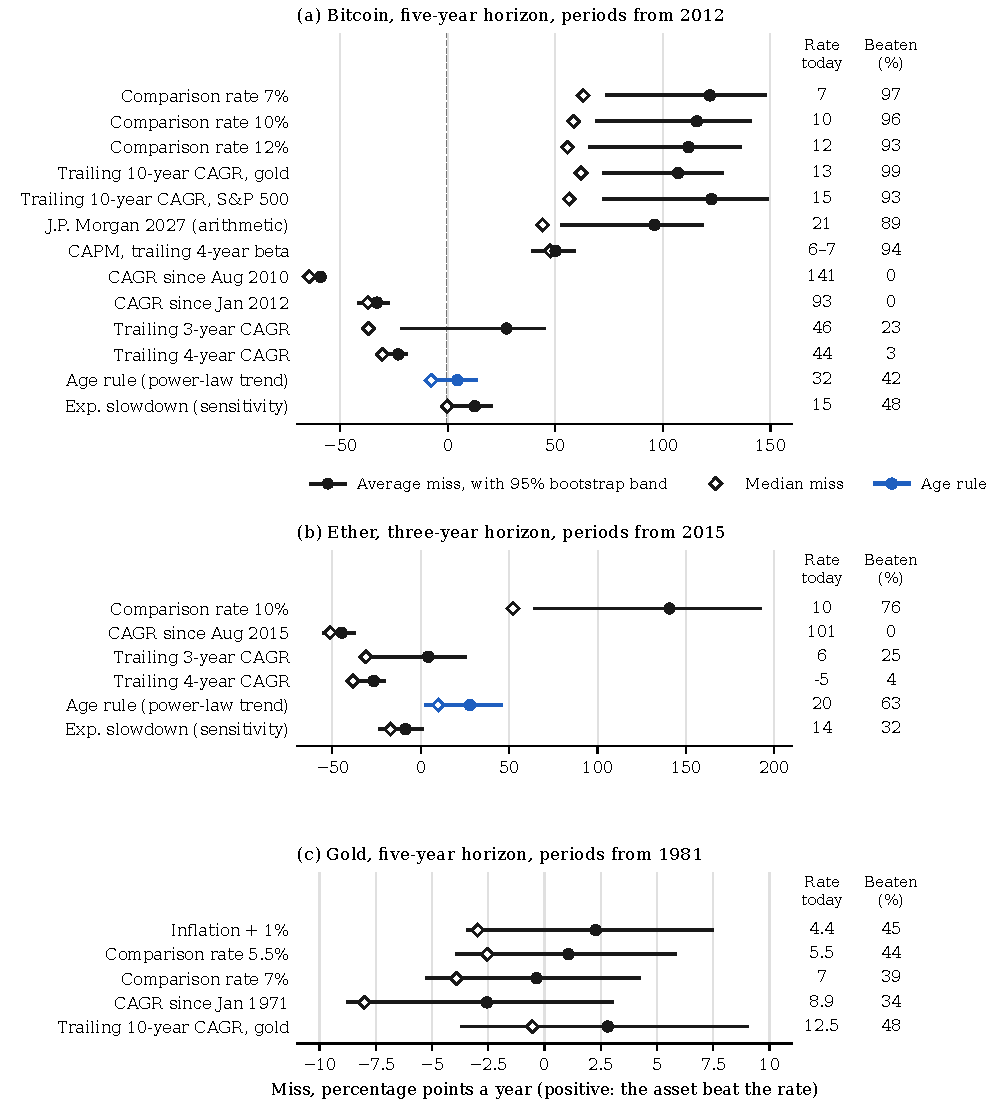
\includegraphics[width=0.95\textwidth]{figs/fig_main.pdf}
\par\smallskip
\begin{minipage}{\textwidth}\footnotesize
\emph{Notes:} Miss: the asset's annual return relative to the rate, $\widehat{G}^{1/h}-1$, in percentage points. For each candidate rate the filled dot is the average miss, $\bar{G}^{1/h}-1$, over rolling $h$-year periods, the quantity a correct expected return sets to zero; the line is its 95\% band from 5,000 stationary-bootstrap resamples of the sequence of $\widehat{G}$ (mean block length equal to the horizon), not the range of outcomes; the hollow diamond is the median miss. The age rule is shown in blue. The columns give the rate the method implies at the end of the sample (September 2026; April 2026 for Ether) and the share of periods in which the asset beat the rate. A band that excludes zero means the data reject the rate: to the right, too low; to the left, too high. A correct expected return has an average miss near zero and is beaten in about 45\% of periods for gold and 17--34\% for Bitcoin (Section~\ref{sec:design}). Periods start in January 2012 (Bitcoin), August 2015 (Ether) and January 1981 (gold) or later. J.P. Morgan: the arithmetic assumption in its 2027 Long-Term Capital Market Assumptions. CAPM: Treasury yield plus trailing four-year beta times a 4\% equity premium, from August 2014. Other horizons, median misses and numbers of periods: Exhibits~\ref{tab:today} and~\ref{tab:calib}.
\end{minipage}
\end{table}

Exhibit~\ref{fig:main} shows, for each way of setting Bitcoin's expected return, how far it missed the returns that followed, what it implies today, and how often it was beaten; panels (b) and (c) do the same for Ether and gold, which Section~\ref{sec:gold} discusses. The methods for Bitcoin span 6\% to 141\% a year, a range that would take Bitcoin's weight in an optimized portfolio from negligible to dominant. The backtest narrows the choice. Ranges in the text cover horizons of three to five years; the figure shows five years for Bitcoin and gold and three for Ether, and Appendix~A.2 reports every horizon.

What would a correct forecast look like in Exhibit~\ref{fig:main}? Three things, each a standard property of an unbiased forecast of a volatile return. The dot should sit at zero with the band straddling it, the condition that the forecast is right on average (Fama and French 2002; Elton 1999). The diamond should sit to the left of the dot, by about half the variance of annual returns, 10--15 points for Bitcoin and a point or so for gold, because the median of a volatile return lies that far below its mean (Jacquier, Kane, and Marcus 2003). And the share of periods beaten should be well under half, 17--34\% for Bitcoin and about 45\% for gold, for the same reason (Appendix~A.3). No candidate for Bitcoin meets all three; the age rule comes closest, and the rest fail badly.

An allocator who had assumed 10\% a year at any point since 2012 would have seen Bitcoin beat that assumption in 94--99\% of the periods that followed, by about 100 points a year on average; even the lower end of the band is above 50 points. J.P. Morgan's 21\% would have been beaten in about nine periods in ten, by 70--95 points a year, and a CAPM rate set in real time did no better. Extrapolating Bitcoin's own past errs the other way: its average growth since 2012 overstated what followed by about 30 points a year, and its growth over the previous four years by 9--23 points. Growth over the previous three years looks right on average only because a handful of spectacular periods carry it; Bitcoin fell short of it in three periods out of four.

Rates that assume growth keeps slowing do far better. Bitcoin beat the power-law rate by just 1--5 points a year on average, well inside a band of roughly $\pm$10 points, and fell short of it in the median period by 4--10 points. It beat the rate in 35--46\% of periods, between the 17--34\% expected of a correct forecast and the 50\% of a median. A typical miss in a single period, about 20 points a year, is half that of the averages. The exponential slowdown, by contrast, was too low: Bitcoin beat it by 5--13 points a year, and at five years the band excludes zero. It also depends on the window used to fit it (Appendix~A.3).

Why does average growth overstate the expected return? For a maturing asset, past growth includes one-off gains that will not recur. Fama and French (2002) show that average equity returns over 1951--2000 far exceeded the expected returns implied by dividend and earnings growth, largely because falling discount rates produced capital gains that nobody expected. Bitcoin's past growth includes a similar gain, its repricing from a fringe asset to a widely held one, and gold's growth since 1971 includes its repricing after the end of dollar convertibility; gold's average growth since 1971 overstated what followed by about 3 points a year. An own-history rate for a maturing asset should therefore assume that growth keeps slowing.

The power-law rate, which came closest, reduces to a simple formula, which we call the \emph{age rule}. With age $A_t$ in years since 3 January 2009, equation~(\ref{eq:powerlaw}) can be written
\begin{equation}
\ln(1+c_{t,h})=\frac{\beta_t}{h}\ln\!\left(1+\frac{h}{A_t}\right)\approx\frac{\beta_t}{A_t}, \label{eq:formula}
\end{equation}
where the approximation holds when the horizon is short relative to the asset's age. In log terms, Bitcoin's expected return is its power-law exponent divided by its age. What it gives falls as Bitcoin ages: $\beta/A$ is 0.32 at age 18 and 0.16 at age 35. As of September 2026, with $\beta=5.62$ and $A=17.7$ years, the age rule's forecast is about 36\% for the year to September 2027 and 32\% a year for the five years to September 2031; if the exponent holds, about 27\% a year from 2030, 22\% from 2035 and 18\% from 2040 (Exhibit~\ref{tab:formula}). The age rule gives an expected return for any horizon. This paper reports the five-year figure because five years is the horizon at which the rule is tested, and uses the one-year figure only where a comparison calls for it (Section~\ref{sec:required}). The 32\% is an arithmetic-type figure; its compound counterpart, from the median miss, is about 22--28\%, above even J.P. Morgan's bull case of 16.6\%, and within the 15--34\% that adoption scenarios currently imply, nearer the top.

The formula is not ours: it is the growth rate of the power law, already fitted, tested and quoted by its followers (Burger 2019; Burger and Vijn 2024; Baquero and Menezes 2026; \c{S}enel and Y{\i}lmaz 2026; Santostasi and Perrenod 2026); what is new is to read it as the expected return, estimate the exponent in real time, and test it as a forecast against the rates practitioners use.

\begin{table}[htbp]
\centering
\caption{The age rule in real time: the exponent fitted each month, the five-year expected return it forecast at that date, and the return that followed.}
\label{tab:formula}
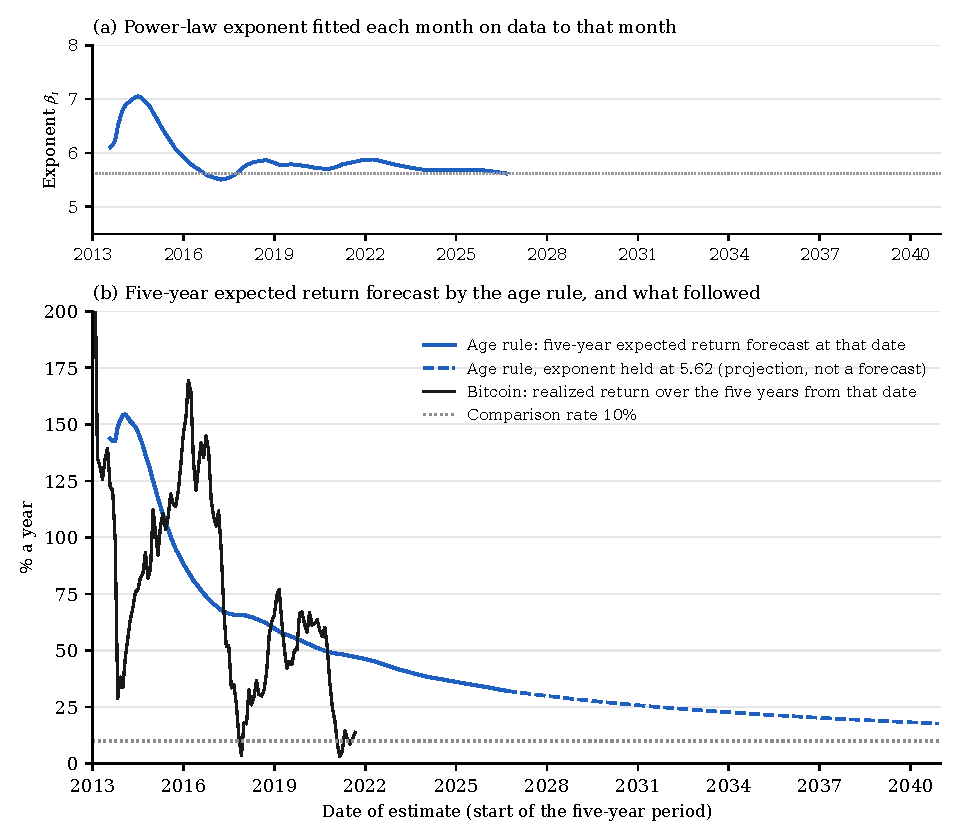
\includegraphics[width=0.95\textwidth]{figs/fig_agerule.pdf}
\par\smallskip
\begin{minipage}{\textwidth}\footnotesize
\emph{Notes:} (a) $\beta_t$, the slope of a least-squares fit of log price on log age using monthly data from August 2010 to the month shown; the dotted line is its September 2026 value, 5.62. (b) The age rule's five-year expected return at each date, $(1+5/A_t)^{\beta_t/5}-1$, using that date's exponent; Bitcoin's realized compound annual return over the five years that followed, available to September 2021; and a 10\% comparison rate. The dashed line holds the exponent at 5.62 and shows what the age rule implies as Bitcoin ages, not a forecast: about 27\% a year from 2030, 22\% from 2035 and 18\% from 2040. Averaged over all periods from 2012, the realized return exceeded the age rule's forecast by 1--5 points a year (Exhibit~\ref{fig:main}).
\end{minipage}
\end{table}

\section{Is the Age Rule Real?}\label{sec:formula}

Critics argue that the power law is a spurious regression (Stolte 2022) or describes the past without constraining the future (Faulkner 2026). Earlier tests of the trend asked whether it tracks the price (Burger and Vijn 2024; Baquero and Menezes 2026; Baquero and Tinoco 2026); the backtest asks whether the growth rate it implies is an unbiased forecast of the return, which a trend that tracks the median path could still misstate. Three facts say the age rule is real. It held up out of sample: in panel (b) of Exhibit~\ref{tab:formula} the five-year return swings far above and below the forecast made at each date and crosses it repeatedly, so that the misses, though large, average out (Section~\ref{sec:calibsec}). The exponent has been stable in real time, at 5.6--5.9 since 2018 (panel (a)), and the returns that followed imply a similar value: regressing realized growth on what the age rule predicts gives 5.2--5.7 and explains 37--69\% of the variation in forward growth, and the exponent's 95\% confidence interval, 5.25--5.99, translates into 30--35\% for the five-year expected return (Appendix~A.3). And prices have reverted to the trend rather than drifted from it: deviations of the log price from the trend are stationary, with a half-life of eight to ten months (Exhibit~\ref{tab:adoption}).

The stricter test uses only the periods that began after the trend's form was published in 2019, since before then only its exponent is estimated without hindsight. In those periods the age rule ran slightly high: Bitcoin fell short of it by 5--8 points a year on average and 9--12 at the median, and beat it in 21--48\% of periods, while a 10\% rate was still beaten by about 30 points a year, J.P. Morgan's 21\% by 15--19, and Bitcoin's average growth since 2012 was too high by about 40 (Exhibit~\ref{tab:postpub}). Those periods span at most one independent five-year stretch, so they show only that the age rule did not break after publication.

The natural explanation is adoption. Under a generalized Metcalfe's law (Metcalfe 2013; Wheatley et al.\ 2019), value rises with a power of the number of users, and Santostasi and Perrenod (2026) derive the price--age power law from the growth of addresses. The evidence depends on how users are counted (Exhibit~\ref{tab:adoption}): price moves together with the number of addresses holding a balance over 2010--2026, as Perrenod (2026) also reports, but less clearly in later subsamples and not with active addresses, which miss coins held by exchanges and funds. Slowing adoption is a plausible explanation, not an established one.

The main uncertainty is the shape of the slowdown. An exponential slowdown, in which growth decays at a constant rate in calendar time rather than in proportion to age, fits the past about as well with two parameters instead of one and implies 15--18\% a year today. We prefer the age rule because its single parameter has been stable, while the exponential rate's half-life of growth has ranged from 2.5 to 7.5 years; because the exponential rate was too low in the backtest; and because, extrapolated, it would put Bitcoin's expected return below 7\% by the mid-2030s, although Bitcoin is nearly four times as volatile as gold. We report it as a sensitivity.

The age rule has limits. Its misses in individual periods are large, about 20 points a year. It is an empirical regularity, proposed with knowledge of Bitcoin's history, although its exponent is estimated in real time. It has no floor, falling to 10\% only in the late 2060s, whereas at some point Bitcoin's expected return must approach that of mature assets. It rests on a history that includes adoption nobody could have foreseen and on an asset studied because it survived, both of which push realized returns above what could have been expected at the time. And it is specific to Bitcoin: the same form was too low for Ether over its short history (Section~\ref{sec:gold}).

\section{Required Return and What Holders Expect}\label{sec:required}

How does 32\% compare with the return Bitcoin's risk requires? A CAPM required return, $r_f+\beta\times\mathit{ERP}$ (Sharpe 1964; Lintner 1965), takes the ten-year Treasury yield, 5.0\% in September 2026, an equity risk premium of 4\% (6\% as a high case) and Bitcoin's beta to the S\&P 500, the usual stand-in for the market portfolio; Bitcoin's own weight in a global portfolio of risky assets is about 1\%, so including it would barely change the beta (Roll 1977). The beta is 0.33 over the last four years, 1.06 since 2016 and 2.12 since 2012 (Appendix~A.3), giving required returns of 6--7\%, 9--11\% and 13--18\%, far below 32\% and close to the 7--21\% rates the backtest rejected. J.P. Morgan's own assumptions, a correlation of 0.33 with US large caps and volatilities of 55\% and 18\%, imply a beta of about 1.0 and the same 9--11\%. For gold, a beta near zero gives about 5\%, close to inflation plus 1\%; for Ether, 13--20\%.

The CAPM is a poor guide to what Bitcoin's holders require. The problem is not the proxy but the premise: the model assumes that the investors who set the price hold the market portfolio and care only about covariance with it, whereas Bitcoin's correlation with the S\&P 500 is below 0.2 and crypto returns follow factors of their own (Liu and Tsyvinski 2021; Liu, Tsyvinski, and Wu 2022); J.P. Morgan keeps Bitcoin out of its main covariance matrices for the same reason, its ``unstable correlations.'' Surveys point the same way: in a large survey of US households, those holding crypto expected it to return 22\% over the next year in 2021 and 14\% in 2025, against 7\% and 5\% for those not holding it (Candia et al.\ 2026). Holders expect, and presumably require, more than the CAPM implies.

Yet holders expected far less than the age rule forecast at the time, about 55\% for the next year in 2021 and 40\% in 2025 (from late 2021 Bitcoin in fact returned about 14\% a year, below both). If their expectations were similar earlier, Bitcoin delivered more over its history than investors required or expected. Whether that came from feared outcomes that did not occur, such as a ban or a collapse in adoption, or from adoption that investors underrated, the backtest cannot tell; in the first case the age rule, fitted to the one path that occurred, overstates the expected return.

No existing model has been asked to explain this gap. The CAPM cannot: the factors that price stocks explain almost none of Bitcoin's returns, so the difference is not a premium on any priced risk. The equilibrium models of Bitcoin's price (Biais et al.\ 2023; Pagnotta 2022; Cong, Li, and Wang 2021) are statements about structure, not level: the price is the discounted value of the benefits of holding and using Bitcoin, so its expected appreciation equals the required return less the yield those benefits provide, as for a commodity with a convenience yield, and the level of the price follows adoption. Their required return is the general form of the CAPM's, a premium for the covariance of Bitcoin's payoff with the investor's marginal utility, which the models leave to be estimated; for a diversified investor it is close to the CAPM's figure or below it, since Bitcoin barely covaries with consumption or the market. The structure therefore makes the gap sharper, not smaller: with a positive benefit yield the price should appreciate by less than a required return that is itself low. But none of the models yields a rate that could enter Exhibit~\ref{fig:main}: Biais et al.\ estimate their pricing equation on past data rather than project a return, and the other two calibrate their models to illustrate the dynamics, not to forecast. None has been calibrated to a long-run required return that could be set against 32\%, and none asks whether a premium for adoption risk accounts for the difference. Rates set at the level of comparable assets are thus doubly flawed: poor forecasts, justified by a view of required returns that does not describe Bitcoin's holders.

\section{Gold and Ether}\label{sec:gold}

Gold is the control: an asset whose expected return is known from a long record, so that the backtest's behaviour on it shows what the test can and cannot do. Over 1836--2011 its real price rose by 1.1\% a year, and its returns barely move with consumption, so its expected return is close to the real risk-free rate, about 1\% above inflation (Barro and Misra 2016). Its real price reverts to its mean, so a high real price has preceded below-average returns (Erb and Harvey 2013); other work links its price to the yield required on stocks (Faug\`{e}re and Van Erlach 2004) or to nominal GDP and financial wealth (World Gold Council 2024). Much of the two-century record comes from the gold standard, when the price was fixed; since dollar convertibility ended, gold has returned 4.8\% a year above US inflation from 1971, a figure that includes its repricing, and 1.5\% from 1981.

The backtest behaves as it should on gold (Exhibit~\ref{fig:main}, panel (c)). Since 1981, every candidate passes: gold's average miss lies between $-3$ points a year for its own growth since 1971, which includes the 1970s repricing, and $+2$ to $+3$ for inflation plus 1\% and its trailing ten-year growth, with 5.5\% and 7\% in between, and every band includes zero. The rates differ by less than gold's returns vary, so 45 years of periods cannot rank them. Since 2012 gold has returned 6.8\% a year against inflation of 2.7\%; whether that reflects a lasting change in demand, such as central-bank buying, or a run that will reverse, the backtest cannot say, and in September 2026 gold's real price was about 1.5 times its 1980 peak. For gold, then, the long record narrows the expected return to about 1--2\% above inflation, 4.4--5.4\% in September 2026, where J.P. Morgan's 5.5\% also sits, with the recent run a reason to show a higher rate as a sensitivity; the backtest confirms that range and shows what a 45-year history can resolve, differences of about five points, not three.

Ether is the same test applied to a younger asset, and its history is too short to say anything firm (panel (b)). As for Bitcoin, the comparison rates were far too low and its average growth far too high, but even the age rule, with Ether's own exponent of about 2.2, was too low, by 28 points a year at three years. Exhibit~\ref{fig:eth} shows why. Ether's exponent has been as stable as Bitcoin's, at 1.9--2.4 since 2018, but the forecasts it gave in 2018--2020 fell far short of the returns that followed, while from 2021 forecast and outcome have tracked each other. Whether the early miss was a one-off repricing, like the one Bitcoin's history contains, or a failure of the form, 57 overlapping periods cannot say. Its trailing three-year growth looks right on average, but only as Bitcoin's did: a few huge periods carry the average, the band is some 60 points wide, and Ether fell short of it in three periods out of four, by 31 points in the median period. The exponential-slowdown rate rests on fewer than two dozen periods. With about three independent three-year periods and annual volatility above 100\%, the backtest cannot bound Ether's expected return.

\begin{table}[htbp]
\centering
\caption{The age rule applied to Ether: the exponent fitted each month and the three-year expected return it forecast, against the return that followed.}
\label{fig:eth}
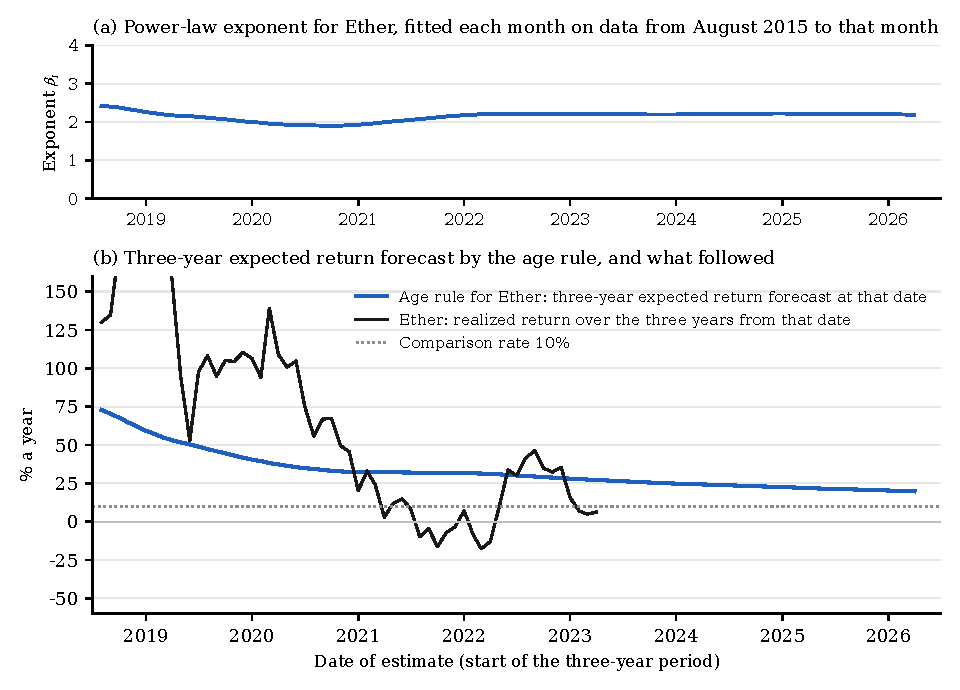
\includegraphics[width=0.95\textwidth]{figs/fig_agerule_eth.pdf}
\par\smallskip
\begin{minipage}{\textwidth}\footnotesize
\emph{Notes:} As Exhibit~\ref{tab:formula}, for Ether, with age counted from 30 July 2015, the exponent fitted on monthly data from August 2015 to the month shown (first fit August 2018, three years of data), and a three-year horizon, the one used for Ether throughout: the forecast is $(1+3/A_t)^{\beta_t/3}-1$ and the realized return the compound annual return over the three years that followed, available to April 2023. Over the 57 periods the forecast averaged 39\% a year and the realized return 65\%.
\end{minipage}
\end{table}

The width of the bands in Exhibit~\ref{fig:main} measures what each history reveals: about $\pm$5 points for gold, $\pm$10 for Bitcoin's age rule, and 20--30 for the rates that come closest for Ether. In these three assets, which all pay no income, precision tracks maturity: the longer the history relative to how fast the expected return is changing, and the less noisy the returns, the more it reveals; three assets are too few to establish maturity as the cause.

\section{Implications for Practice}\label{sec:practice}

Four points follow for capital market assumptions.

\begin{enumerate}
\item \emph{For Bitcoin, use the age rule, with a time path and a sensitivity.} Applied today, it forecasts about 32\% a year for September 2026 to 2031 and, if the exponent holds, 27\% from 2030, 22\% from 2035 and 18\% from 2040 (Exhibit~\ref{tab:formula}). Show allocations also at the 15--18\% of an exponential slowdown, the stress test against a bear case that J.P. Morgan recommends for any Bitcoin allocation. Do not use a rate at equity-like levels, however it is derived, and do not extrapolate long-run average growth: the first was beaten in about nine periods in ten, the second in almost none. The 32\% is a mean rate, the right one for an expected price; a trend line fitted to log prices calls for the median rate, about 12 points lower.
\item \emph{Check an assumption against the average return that followed, not against how often it was beaten.} For a volatile asset the mean return lies well above the median, so a correct expected return for Bitcoin is beaten in only a fifth to a third of periods. An assumption that Bitcoin beat half the time was therefore too low, and one it beat nine times in ten far too low.
\item \emph{Do not take Bitcoin's required return from the CAPM.} The CAPM gives 6--18\% depending on the window used for beta, and its premise does not describe Bitcoin's holders, who report expecting 14--22\% a year. Investors who expect less than the age rule may be pricing risks that have not materialized, so an allocation should say whether it adopts the age rule as the expected return or discounts it for such risks.
\item \emph{For gold, start from inflation plus 1--2\%, with a higher rate as a sensitivity; for Ether, treat any assumption as provisional.} Gold's long record and its CAPM rate agree on about 4.4--5.4\% in 2026, and a rate near 7\% belongs in the sensitivity analysis. For Ether the methods imply anywhere from $-5$\% to 101\% a year, and none can yet be trusted.
\end{enumerate}

\section{Conclusion}\label{sec:conclusion}

The rates institutions use for Bitcoin's long-run expected return fail as forecasts, and Bitcoin's own long-run average growth fails the other way. A rule implicit in Bitcoin's power-law price trend, its exponent divided by its age, comes closest: it matched the returns that followed on average over 2012--2026, ran a few points high in the periods since the trend was published, and today forecasts about 32\% a year for September 2026 to 2031, less as Bitcoin ages. Gold, whose expected return is known from two centuries of data, shows the test working: every candidate within three points of that figure passes, and the Bitcoin rejections lie far outside any such margin. Ether shows the test's limit: ten years of history validate no rule, the age rule included.

The open question is the gap between that 32\% and what Bitcoin's risk requires. The CAPM gives 6--18\%, holders report expecting 14--22\%, and Bitcoin has delivered more than either. Whether the difference is compensation for risks that have not yet materialized, such as a ban or a collapse in adoption, or the mark of an asset the market has underpriced, realized returns cannot say, and no existing model has been asked: the CAPM does not fit Bitcoin's holders, and the equilibrium models of its price have not been calibrated to a long-run required return. This paper supplies the inputs such a calibration has to fit: a tested expected return, a CAPM required return, and what holders say they expect. The evidence rests on few independent periods and on an asset studied because it survived, and should be revisited as the history of cryptoassets lengthens.

\section*{Disclaimer}

This research was conducted independently and without funding, review, or endorsement. The views expressed are solely those of the author and do not represent any institutional position. This paper is for informational and academic purposes only and does not constitute financial, investment, tax, or legal advice, nor a recommendation to buy or sell any financial instrument. Any illustrative data used are from publicly available sources.

\section*{References}
\begingroup
\small
\setlength{\parindent}{-1.5em}\setlength{\leftskip}{1.5em}\setlength{\parskip}{0.3em}\sloppy

\chg{Baquero, C., and R. Menezes. 2026. ``Bitcoin's Power Law: Weak Structure, Strong Forecasts.'' arXiv preprint 2605.21316. \url{https://arxiv.org/abs/2605.21316}.}

\chg{Baquero, C., and D. Tinoco. 2026. ``The Naive--Power Law Blend as a Robust Baseline for Bitcoin Price Forecasting.'' \emph{Digital Finance} 8: 60.}

\chg{Barro, R. J., and S. P. Misra. 2016. ``Gold Returns.'' \emph{Economic Journal} 126 (594): 1293--1317.}

\chg{Biais, B., C. Bisi\`{e}re, M. Bouvard, C. Casamatta, and A. J. Menkveld. 2023. ``Equilibrium Bitcoin Pricing.'' \emph{Journal of Finance} 78 (2): 967--1014.}

\chg{Bitwise Asset Management. 2026. ``Bitcoin 2027 Long-Term Capital Market Assumptions.'' October 2026. \url{https://static.bitwiseinvestments.com/Research/Bitwise-Bitcoin-Long-Term-Capital-Market-Assumptions-2027.pdf}.}

\chg{Black, F., and R. Litterman. 1992. ``Global Portfolio Optimization.'' \emph{Financial Analysts Journal} 48 (5): 28--43.}

\chg{Burger, H. C. 2019. ``Bitcoin's Natural Long-Term Power-Law Corridor of Growth.'' \emph{Coinmonks} (Medium). \url{https://medium.com/coinmonks/bitcoins-natural-long-term-power-law-corridor-of-growth-649d0e9b3c94}.}

\chg{Burger, H. C., and P. Vijn. 2024. ``Bitcoin's Time-Based Power-Law and Cointegration Revisited.'' \emph{Quantodian} (Medium), January 31, 2024. \url{https://medium.com/quantodian-publications/bitcoins-time-based-power-law-and-cointegration-revisited-15f212b95ea5}.}

\chg{Candia, B., O. Coibion, Y. Gorodnichenko, and M. Weber. 2026. ``Do You Even Crypto, Bro? Cryptocurrencies in Household Finance.'' Working Paper 26-16, Federal Reserve Bank of Cleveland.}

\chg{Coin Metrics. 2026. ``Community Network Data: \texttt{btc.csv} and \texttt{eth.csv}.'' GitHub repository \texttt{coinmetrics/data}. Accessed October 31, 2026.}

Cong, L. W., \chg{Y. Li, and N. Wang}. 2021. ``Tokenomics: Dynamic Adoption and Valuation.'' \emph{Review of Financial Studies} 34 (3): 1105--1155.

\chg{DataHub. 2026a. ``Gold Prices.'' Monthly USD prices from the World Bank Commodity Markets (``Pink Sheet'') from 1960. GitHub repository \texttt{datasets/gold-prices}. Accessed October 31, 2026.}

\chg{DataHub. 2026b. ``S\&P 500.'' Monthly data compiled from R. J. Shiller's data, extended with FRED index levels after June 2023. GitHub repository \texttt{datasets/s-and-p-500}. Accessed October 31, 2026.}

\chg{Dickey, D. A., and W. A. Fuller. 1979. ``Distribution of the Estimators for Autoregressive Time Series with a Unit Root.'' \emph{Journal of the American Statistical Association} 74 (366): 427--431.}

\chg{Elton, E. J. 1999. ``Expected Return, Realized Return, and Asset Pricing Tests.'' \emph{Journal of Finance} 54 (4): 1199--1220.}

\chg{Engle, R. F., and C. W. J. Granger. 1987. ``Co-Integration and Error Correction: Representation, Estimation, and Testing.'' \emph{Econometrica} 55 (2): 251--276.}

\chg{Erb, C. B., and C. R. Harvey. 2013. ``The Golden Dilemma.'' \emph{Financial Analysts Journal} 69 (4): 10--42.}

\chg{Fama, E. F., and K. R. French. 1997. ``Industry Costs of Equity.'' \emph{Journal of Financial Economics} 43 (2): 153--193.}

\chg{Fama, E. F., and K. R. French. 2002. ``The Equity Premium.'' \emph{Journal of Finance} 57 (2): 637--659.}

\chg{Faug\`{e}re, C., and J. Van Erlach. 2004. ``The Price of Gold: A Global Required Yield Theory.'' Working paper, Finance 0403003, University Library of Munich. \url{https://ideas.repec.org/p/wpa/wuwpfi/0403003.html}.}

\chg{Faulkner, P. 2026. ``Description Without Prediction: A Methodological Critique of Bitcoin Price Power Law Models.'' Working paper, Zenodo. \url{https://zenodo.org/records/19975701}.}

\chg{Federal Reserve Bank of St.\ Louis. 2026. ``Federal Reserve Economic Data (FRED): Consumer Price Index for All Urban Consumers, All Items in U.S. City Average (CPIAUCNS), 10-Year Treasury Constant Maturity Rate (GS10), and S\&P 500 (SP500).'' Accessed November 3, 2026. \url{https://fred.stlouisfed.org}.}

\chg{ff137. 2026. ``Bitstamp BTC/USD 1-Minute OHLC Data.'' GitHub repository \texttt{ff137/bitstamp-btcusd-minute-data}. Accessed October 31, 2026.}

\chg{J.P. Morgan Asset Management. 2026. ``2027 Long-Term Capital Market Assumptions.'' 31st ed., October 2026, 46--47. \url{https://am.jpmorgan.com/us/en/asset-management/gim/adv/ltcma}.}

\chg{Jacquier, E., A. Kane, and A. J. Marcus. 2003. ``Geometric or Arithmetic Mean: A Reconsideration.'' \emph{Financial Analysts Journal} 59 (6): 46--53.}

\chg{Kwiatkowski, D., P. C. B. Phillips, P. Schmidt, and Y. Shin. 1992. ``Testing the Null Hypothesis of Stationarity against the Alternative of a Unit Root: How Sure Are We That Economic Time Series Have a Unit Root?'' \emph{Journal of Econometrics} 54 (1--3): 159--178.}

Lintner, J. 1965. ``The Valuation of Risk Assets and the Selection of Risky Investments in Stock Portfolios and Capital Budgets.'' \emph{Review of Economics and Statistics} 47 (1): 13--37.

\chg{Liu, Y., and A. Tsyvinski. 2021. ``Risks and Returns of Cryptocurrency.'' \emph{Review of Financial Studies} 34 (6): 2689--2727.}

\chg{Liu, Y., A. Tsyvinski, and X. Wu. 2022. ``Common Risk Factors in Cryptocurrency.'' \emph{Journal of Finance} 77 (2): 1133--1177.}

\chg{Metcalfe, B. 2013. ``Metcalfe's Law after 40 Years of Ethernet.'' \emph{Computer} 46 (12): 26--31.}

\chg{Newey, W. K., and K. D. West. 1987. ``A Simple, Positive Semi-Definite, Heteroskedasticity and Autocorrelation Consistent Covariance Matrix.'' \emph{Econometrica} 55 (3): 703--708.}

\chg{Pagnotta, E. S. 2022. ``Decentralizing Money: Bitcoin Prices and Blockchain Security.'' \emph{Review of Financial Studies} 35 (2): 866--907.}

\chg{Papadogiannis, A. 2026a. ``A Dual-Risk Theory of Valuation Separating Market-Based Discounting from Expectational Distortion.'' \emph{Discover Analytics} 4 (1): 19.}

Papadogiannis, A. 2026b. ``From Unified Discounting to Dual-Risk: A New Lens on DCF Valuation.'' \emph{Finance Research Open} 2: 100096.

\chg{Papadogiannis, A. 2027. ``Beyond Discount Rates: A Valuation Framework for Unpriced Systematic Risk.'' \emph{Journal of Investing}, forthcoming.}

\chg{Perrenod, S. 2026. ``Does Bitcoin Really Follow Metcalfe's Law? Five New Tests.'' \emph{Money or Debt} (Substack), August 21, 2026. \url{https://stephenperrenod.substack.com/p/does-bitcoin-really-follow-metcalfes}.}

\chg{PlanB. 2019. ``Modeling Bitcoin's Value with Scarcity.'' Medium, March 22, 2019. \url{https://medium.com/@100trillionUSD/modeling-bitcoins-value-with-scarcity-91fa0fc03e25}.}

\chg{Politis, D. N., and J. P. Romano. 1994. ``The Stationary Bootstrap.'' \emph{Journal of the American Statistical Association} 89 (428): 1303--1313.}

\chg{Roll, R. 1977. ``A Critique of the Asset Pricing Theory's Tests Part I: On Past and Potential Testability of the Theory.'' \emph{Journal of Financial Economics} 4 (2): 129--176.}

\chg{Santostasi, G., and S. Perrenod. 2026. ``A Mechanistic Derivation of the Bitcoin Price Power Law: Network Adoption Dynamics and Generalised Metcalfe Scaling.'' Working paper, Zenodo.}

\chg{Selby, G. 2025. ``Building Bitcoin Capital Market Assumptions.'' CF Benchmarks, December 18, 2025. \url{https://www.cfbenchmarks.com/blog/building-bitcoin-capital-market-assumptions}.}

\chg{\c{S}enel, \.{I}. K., and F. Y{\i}lmaz. 2026. ``Bitcoin Valuation through Power Law Analysis: Evidence for Long-Term Mean Reversion and Short-Term Momentum.'' \emph{Journal of Business Economics and Finance} 15 (1): 65--77.}

Sharpe, W. F. 1964. ``Capital Asset Prices: A Theory of Market Equilibrium under Conditions of Risk.'' \emph{Journal of Finance} 19 (3): 425--442.

\chg{Sigel, M. 2026. ``Bitcoin Long-Term Capital Market Assumptions.'' VanEck, January 8, 2026. \url{https://www.vaneck.com/us/en/blogs/digital-assets/matthew-sigel-vaneck-bitcoin-long-term-capital-market-assumptions/}.}

\chg{Stolte, T. 2022. ``Bitcoin's Power-Law Corridor Debunked.'' Amdax Asset Management (Medium), September 2, 2022. \url{https://medium.com/amdax-asset-management/bitcoins-power-law-corridor-debunked-1b40783657bf}.}

\chg{Wheatley, S., D. Sornette, T. Huber, M. Reppen, and R. N. Gantner. 2019. ``Are Bitcoin Bubbles Predictable? Combining a Generalized Metcalfe's Law and the Log-Periodic Power Law Singularity Model.'' \emph{Royal Society Open Science} 6 (6): 180538.}

\chg{World Gold Council. 2024. ``Gold's Long-Term Expected Return (GLTER).'' Goldhub research, October 17, 2024. \url{https://www.gold.org/goldhub/research/golds-long-term-expected-return-glter}.}
\par\endgroup

% ============================ APPENDICES ============================
\appendix
\renewcommand{\thesection}{\Alph{section}}

% ============================ NEW APPENDIX D ============================
\Needspace{14\baselineskip}
\section{\texorpdfstring{\chg{Data Sources and Robustness Results}}{Data Sources and Robustness Results}}
\setcounter{figure}{0}\renewcommand{\thefigure}{A\arabic{figure}}\renewcommand{\thetable}{A\arabic{figure}}
\begingroup\color{blue}

\subsection*{A.1 Data}

All data files, the scripts that produce every exhibit and the results they generate are available at \url{https://github.com/apapadogiannis/bitcoin-age-rule} and archived on Zenodo, \url{https://doi.org/10.5281/zenodo.24004326}.

\begin{table}[H]
\centering\color{blue}
\caption{Data sources and construction.}
\label{tab:D1}
\footnotesize
\begin{tabularx}{\textwidth}{>{\raggedright\arraybackslash}p{2.4cm}>{\raggedright\arraybackslash}p{2.6cm}>{\raggedright\arraybackslash}X}
\toprule
Series & Sample & Source and construction\\
\midrule
Bitcoin & Aug 2010--Sep 2026 & Month-end close of Bitstamp BTC/USD one-minute candles from January 2012 (ff137 2026); Coin Metrics reference price before 2012 (Coin Metrics 2026). Over 2012--2026 the two sources' month-end prices differ by a median of 0.1\% and at most 4.3\%.\\
Ether & Aug 2015--Apr 2026 & Coin Metrics reference price, month-end (Coin Metrics 2026).\\
\chg{Bitcoin addresses} & \chg{Aug 2010--Apr 2026} & \chg{Monthly means of daily counts of addresses with a non-zero balance and of active addresses (Coin Metrics 2026).}\\
Gold & Jan 1971--Sep 2026 & Monthly average price, USD per ounce, World Bank Commodity Markets (DataHub 2026a).\\
S\&P 500 TR & Jan 1871--Sep 2026 & Shiller monthly price and dividends (DataHub 2026b), total return accrued monthly at the prevailing dividend yield; after June 2023, index levels from FRED (Federal Reserve Bank of St.\ Louis 2026) with a dividend yield of 1.3\%.\\
\chg{Ten-year Treasury yield} & \chg{Jan 1871--Sep 2026} & \chg{Shiller long-term interest rate (DataHub 2026b) to December 2022, FRED series GS10 (Federal Reserve Bank of St.\ Louis 2026) from January 2023.}\\
\chg{US consumer prices} & \chg{Jan 1971--Sep 2026} & \chg{Consumer price index for all urban consumers, not seasonally adjusted: Shiller series (DataHub 2026b) to December 2022, FRED series CPIAUCNS (Federal Reserve Bank of St.\ Louis 2026) from January 2023; October 2025, not published, interpolated.}\\
\bottomrule
\end{tabularx}
\end{table}

\subsection*{A.2 Full backtest results}

Exhibit~\ref{tab:today} gives, for every candidate rate for Bitcoin and every horizon, the numbers summarized in Exhibit~\ref{fig:main}; Exhibit~\ref{tab:calib} does the same for Ether and gold.

\begin{table}[H]
\centering
\caption{What each method implies for Bitcoin's expected return in September 2026, and its record as a forecast at each horizon.}
\label{tab:today}
\footnotesize\setlength{\tabcolsep}{2pt}
\begin{tabular}{lr@{\hspace{4pt}}rrr@{\hspace{4pt}}rrr@{\hspace{4pt}}rrr}
\toprule
 & Rate, Sept & \multicolumn{3}{c}{Average miss (\%)} & \multicolumn{3}{c}{Median miss (\%)} & \multicolumn{3}{c}{Beaten (\%)}\\
\cmidrule(lr){3-5}\cmidrule(lr){6-8}\cmidrule(lr){9-11}
Method & 2026 (\%) & $h=3$ & $h=4$ & $h=5$ & $h=3$ & $h=4$ & $h=5$ & $h=3$ & $h=4$ & $h=5$\\
\midrule
Comparison rate 7\% & 7 & $+$103 & $+$95 & $+$122 & $+$59 & $+$68 & $+$63 & 96 & 100 & 97 \\
Comparison rate 10\% & 10 & $+$98 & $+$90 & $+$116 & $+$54 & $+$64 & $+$59 & 94 & 99 & 96 \\
Comparison rate 12\% & 12 & $+$94 & $+$86 & $+$112 & $+$52 & $+$61 & $+$56 & 94 & 98 & 93 \\
Trailing 10-year CAGR, gold & 13 & $+$96 & $+$86 & $+$107 & $+$59 & $+$66 & $+$62 & 97 & 100 & 99 \\
Trailing 10-year CAGR, S\&P 500 TR & 15 & $+$102 & $+$95 & $+$123 & $+$54 & $+$66 & $+$57 & 93 & 95 & 93 \\
J.P.\ Morgan 2027 CMA (arithmetic) & 21 & $+$80 & $+$72 & $+$96 & $+$40 & $+$49 & $+$44 & 91 & 92 & 89 \\
CAPM, trailing 4-year beta & 6--7 & $+$65 & $+$47 & $+$50 & $+$44 & $+$42 & $+$48 & 96 & 100 & 94 \\
CAGR since Aug 2010 & 141 & $-$56 & $-$60 & $-$59 & $-$59 & $-$62 & $-$64 & 0 & 0 & 0 \\
CAGR since Jan 2012 & 93 & $-$30 & $-$35 & $-$33 & $-$37 & $-$41 & $-$37 & 5 & 0 & 0 \\
Trailing 3-year CAGR & 46 & $+$2 & $+$15 & $+$27 & $-$19 & $-$32 & $-$37 & 30 & 25 & 23 \\
Trailing 4-year CAGR & 44 & $-$9 & $-$17 & $-$23 & $-$21 & $-$27 & $-$30 & 23 & 9 & 3 \\
Age rule (power-law trend) & 32--34 & $+$4 & $+$1 & $+$5 & $-$4 & $-$10 & $-$8 & 46 & 35 & 42 \\
Exp.\ slowdown (sensitivity) & 15--18 & $+$5 & $+$6 & $+$13 & $-$4 & $-$6 & 0 & 43 & 39 & 48 \\
\bottomrule
\end{tabular}
\par\smallskip
\begin{minipage}{\textwidth}\footnotesize
\emph{Notes:} Rate implied: the expected return each method gives with data to September 2026; where it depends on the horizon, the range covers $h=3$ to 5 years. These are what the methods imply, not forecasts. Average miss, median miss and beaten: backtest results for horizons of $h=3$, 4 and 5 years, over periods starting in January 2012 or later, as defined in Exhibit~\ref{tab:calib}; positive misses mean Bitcoin beat the rate. A correctly set expected return has an average miss near zero and, for Bitcoin, is beaten in about 17--34\% of periods (Section~\ref{sec:design}). J.P. Morgan: the arithmetic return assumption in its 2027 Long-Term Capital Market Assumptions (J.P. Morgan Asset Management 2026). CAPM: ten-year Treasury yield plus the trailing four-year beta to the S\&P 500 times an equity risk premium of 4\% (6\% for the upper end of the September 2026 rate); its backtest starts in August 2014, when four years of returns are first available. With windows of three to five years, the exponential-slowdown rate implies 14--18\% as of September 2026.
\end{minipage}
\end{table}

\begin{table}[H]
\centering
\caption{How far each assumed rate for Ether and gold missed the return that followed.}
\label{tab:calib}
\footnotesize\setlength{\tabcolsep}{2.4pt}
\textit{Panel B: Ether, $h=3$}\\[2pt]
\begin{tabular}{lrrrrr}
\toprule
 & & \multicolumn{2}{c}{Miss (\%)} & Beaten & Abs.\\
\cmidrule(lr){3-4}
Assumed rate & $n$ & Average & Median & (\%) & (\%)\\
\midrule
Comparison: 10\% & 93 & $+$141 & $+$52 & 76 & 83 \\
CAGR since Aug 2015 & 57 & $-$45 & $-$51 & 0 & 51 \\
Trailing 3-year CAGR & 57 & $+$4 & $-$31 & 25 & 42 \\
Trailing 4-year CAGR & 45 & $-$27 & $-$38 & 4 & 34 \\
Power-law trend & 57 & $+$28 & $+$10 & 63 & 32 \\
Exp.\ slowdown, 4-year window & 22 & $-$9 & $-$17 & 32 & 23 \\
\bottomrule
\end{tabular}

\medskip
\textit{Panel C: Gold}\\[2pt]
\begin{tabular}{lrrrrr@{\hspace{6pt}}rrrrr}
\toprule
 & \multicolumn{5}{c}{$h=3$} & \multicolumn{5}{c}{$h=5$}\\
\cmidrule(lr){2-6}\cmidrule(lr){7-11}
 & & \multicolumn{2}{c}{Miss (\%)} & Beaten & Abs. & & \multicolumn{2}{c}{Miss (\%)} & Beaten & Abs.\\
\cmidrule(lr){3-4}\cmidrule(lr){8-9}
Assumed rate & $n$ & Average & Median & (\%) & (\%) & $n$ & Average & Median & (\%) & (\%)\\
\midrule
Inflation $+$ 1\% & 513 & $+$2 & $-$1 & 47 & 10 & 489 & $+$2 & $-$3 & 45 & 8 \\
Comparison: 5.5\% & 513 & $+$1 & $-$2 & 43 & 9 & 489 & $+$1 & $-$3 & 44 & 7 \\
Comparison: 7\% & 513 & 0 & $-$4 & 40 & 9 & 489 & 0 & $-$4 & 39 & 7 \\
CAGR since Jan 1971 & 513 & $-$3 & $-$6 & 36 & 11 & 489 & $-$3 & $-$8 & 34 & 10 \\
10-year CAGR, gold & 513 & $+$2 & $+$2 & 54 & 11 & 489 & $+$3 & $-$1 & 48 & 10 \\
\bottomrule
\end{tabular}
\par\smallskip
\begin{minipage}{\textwidth}\footnotesize
\emph{Notes:} Miss: the asset's annual return relative to the rate, $(1+g_{t,h})/(1+c)-1=\widehat{G}^{1/h}-1$; positive means the asset beat the rate. Average: $\bar{G}^{1/h}-1$, where $\bar{G}$ is the average of $\widehat{G}$ across periods; it is close to zero for a correctly set expected return. Median: median miss across periods. Beaten: percentage of periods in which the asset returned more than the rate; for a correctly set expected return it is below 50\% (Section~\ref{sec:design}). Abs.: mean absolute miss, a measure of precision. Power-law trend: fitted to date; Exp.\ slowdown: exponential slowdown; 10-year CAGR: trailing ten-year CAGR at the start of each period; Inflation $+$ 1\%: trailing ten-year US consumer price inflation plus 1\%; 5.5\%: about gold's CAPM rate and J.P. Morgan's assumption. Ether periods start in August 2015 or later and gold periods in January 1981 or later, the first month with a trailing ten-year gold rate; $n$ is the number of periods for which the rate is defined.
\end{minipage}
\end{table}

\subsection*{A.3 Statistical details}

\emph{Share of periods beaten.} If log returns are normal with annual volatility $\sigma$, a correct expected return is beaten with probability $1-\Phi(\sigma\sqrt{h}/2)$; $\sigma$ is 0.11--0.12 for gold and the S\&P 500 since 2012, 0.86 for Bitcoin since 2012 and 0.47 over the last four years, giving about 45\% for gold and 17--34\% for Bitcoin at $h=3$ to 5. The median return lies below the expected return by a factor $e^{\sigma^2/2}$, about 12\% a year for Bitcoin at $\sigma=0.47$.

\emph{Bootstrap bands.} Each band is the 2.5th and 97.5th percentile of the average miss across 5,000 stationary-bootstrap resamples (Politis and Romano 1994) of the monthly sequence of $\widehat{G}$, with mean block length equal to the horizon; doubling the block length changes the bands little.

\emph{Exponential-slowdown rate.} The rate fits an exponential decline to the asset's trailing annualized log growth over a window of $L$ years, $\gamma_s$: it estimates $\ln\gamma_s=a_t+b_t s$ on $s\le t$, with time in years, and sets $c^{\mathrm{ED}}_{t,h}=\exp\{\exp[a_t+b_t(t+h/2)]\}-1$, the growth the fitted decline implies at the middle of the horizon. The main text uses $L=4$. The result depends on the window: with $L=3$ the rate is far too low (Bitcoin beat it by 30 and 53 points a year on average at $h=3$ and 5), with $L=5$ it is about right at five years ($+3$) and slightly high at three ($-4$).

\emph{Age-rule exponent.} Regressing realized forward log growth, $\ln(1+g_{t,h})$, on $\ln(1+h/A_t)/h$ without a constant gives 5.2--5.7 for $h=3$ to 5 ($R^2$ of 0.37--0.69). The 95\% confidence interval for the exponent fitted to September 2026, 5.25--5.99, uses standard errors robust to the persistence of deviations from trend (Newey and West 1987). An exponential slowdown fitted to the same forward growth has $R^2$ of 0.38--0.73.

\emph{CAPM required return.} $r_f$ is the ten-year Treasury yield (Exhibit~\ref{tab:D1}); betas are from monthly simple returns on the S\&P 500 total-return index: 0.33 for Bitcoin over the last four years, 1.06 since 2016 and 2.12 since 2012, with correlations of 0.07--0.18; 2.2--2.6 for Ether; and $-0.04$ to 0.16 for gold. The real-time CAPM rate in Exhibit~\ref{tab:today} uses a trailing four-year beta and an equity risk premium of 4\%.


\subsection*{A.4 Price, age and adoption}

\begin{table}[H]
\centering
\caption{Is the age rule a spurious fit? Price, age and adoption.}
\label{tab:adoption}
\footnotesize\setlength{\tabcolsep}{4pt}
\begin{tabular}{lrrr}
\toprule
Sample start (end April 2026) & Aug 2010 & Jan 2012 & Jan 2016\\
\midrule
\multicolumn{4}{l}{\textit{Price on age:} $\ln P=\alpha+\beta\ln A$}\\
\quad Exponent $\beta$ & 5.65 & 5.61 & 5.67 \\
\quad $R^2$ & 0.96 & 0.94 & 0.88 \\
\quad ADF test on deviations, $p$-value & $<$0.01 & $<$0.01 & 0.03 \\
\quad KPSS test on deviations, $p$-value & $\geq$0.10 & $\geq$0.10 & $\geq$0.10 \\
\quad Half-life of deviations (months) & 8 & 9 & 10 \\
\addlinespace
\multicolumn{4}{l}{\textit{Holder addresses (non-zero balance):} $\ln N=a+b\ln A$; $\ln P=c+d\ln N$}\\
\quad Adoption exponent $b$ (95\% CI) & 3.06 (2.79--3.32) & 2.83 (2.61--3.06) & 2.04 (1.64--2.43) \\
\quad ADF test on deviations of $\ln N$, $p$-value & 0.06 & 0.84 & $<$0.01 \\
\quad Network exponent $d$ (95\% CI) & 1.81 (1.65--1.98) & 1.94 (1.71--2.17) & 2.77 (2.50--3.04) \\
\quad Engle--Granger test of no cointegration, $p$-value & $<$0.01 & 0.06 & 0.18 \\
\addlinespace
\multicolumn{4}{l}{\textit{Active addresses:} $\ln N=a+b\ln A$; $\ln P=c+d\ln N$}\\
\quad Adoption exponent $b$ (95\% CI) & 2.60 (1.97--3.22) & 1.99 (1.39--2.58) & 0.40 (0.01--0.80) \\
\quad ADF test on deviations of $\ln N$, $p$-value & 0.90 & 0.88 & 0.17 \\
\quad Network exponent $d$ (95\% CI) & 1.90 (1.60--2.20) & 2.30 (2.01--2.60) & 4.24 (1.67--6.82) \\
\quad Engle--Granger test of no cointegration, $p$-value & 0.67 & 0.90 & 0.93 \\
\bottomrule
\end{tabular}
\par\smallskip
\begin{minipage}{\textwidth}\footnotesize
\emph{Notes:} $P$: Bitcoin month-end price; $A$: age in years since 3 January 2009; $N$: monthly mean of daily counts of addresses with a non-zero balance (holder addresses) or of active addresses (Coin Metrics 2026). Address data end in April 2026. Confidence intervals use standard errors robust to autocorrelation (Newey and West 1987, 12 lags). ADF: augmented Dickey--Fuller test (Dickey and Fuller 1979) of a unit root in the regression deviations, lag length chosen by the Akaike criterion; KPSS: test of stationarity (Kwiatkowski et al.\ 1992), whose $p$-value is reported only up to 0.10; Engle--Granger: test of no cointegration (Engle and Granger 1987) between $\ln P$ and $\ln N$. The product $b\times d$ is not reported because it is close to $\beta$ almost by construction when both regressions fit closely. Fitted in real time on data from August 2010, the adoption exponent fell from 3.5 in January 2016 to 3.1 in January 2026 for holder addresses and from 4.2 to 2.6 for active addresses.
\end{minipage}
\end{table}

\subsection*{A.5 Periods beginning after the power law was published}

\begin{table}[H]
\centering
\caption{Record of each rate in periods beginning January 2020 or later.}
\label{tab:postpub}
\footnotesize\setlength{\tabcolsep}{5pt}
\begin{tabular}{llrrrrr}
\toprule
 & & & \multicolumn{2}{c}{Miss (\%)} & Beaten & Abs.\\
\cmidrule(lr){4-5}
Horizon & Assumed rate & $n$ & Average & Median & (\%) & (\%)\\
\midrule
$h=3$ & Comparison: 10\% & 45 & $+$27 & $+$23 & 89 & 25 \\
 & J.P.\ Morgan: 21\% & 45 & $+$16 & $+$12 & 78 & 17 \\
 & CAGR since Jan 2012 & 45 & $-$39 & $-$43 & 0 & 42 \\
 & Trailing 4-year CAGR & 45 & $-$9 & $-$22 & 24 & 27 \\
 & Age rule (power-law trend) & 45 & $-$6 & $-$12 & 27 & 15 \\
\addlinespace
$h=4$ & Comparison: 10\% & 33 & $+$27 & $+$19 & 97 & 23 \\
 & J.P.\ Morgan: 21\% & 33 & $+$15 & $+$8 & 70 & 15 \\
 & CAGR since Jan 2012 & 33 & $-$43 & $-$48 & 0 & 45 \\
 & Trailing 4-year CAGR & 33 & $-$21 & $-$27 & 6 & 27 \\
 & Age rule (power-law trend) & 33 & $-$8 & $-$12 & 21 & 13 \\
\addlinespace
$h=5$ & Comparison: 10\% & 21 & $+$31 & $+$23 & 81 & 25 \\
 & J.P.\ Morgan: 21\% & 21 & $+$19 & $+$12 & 57 & 20 \\
 & CAGR since Jan 2012 & 21 & $-$42 & $-$47 & 0 & 46 \\
 & Trailing 4-year CAGR & 21 & $-$31 & $-$36 & 0 & 36 \\
 & Age rule (power-law trend) & 21 & $-$5 & $-$9 & 48 & 15 \\
\bottomrule
\end{tabular}
\par\smallskip
\begin{minipage}{\textwidth}\footnotesize
\emph{Notes:} As in Exhibit~\ref{tab:calib}, for Bitcoin periods beginning in January 2020 or later, after the power-law trend was published (Burger 2019). The periods overlap and span at most one independent five-year period, so no bootstrap band is reported.
\end{minipage}
\end{table}


\endgroup

\end{document}
